\chapter{Implementation}
\label{imp}
\textit{In the this chapter features of the PARROT will be presented. The source code associated with the software will be presented and described as well. The software is based on the previously analyzed design and calculations. So far it has been described how the model is supposed to work, and now the software implementation will be described in detail.}\\
\\
The features will be described, first as the problem that spurred the feature, and then the solution we thought up. 
We will then describe how the solution is executed in the PARROT using code segments. Finally we will present notes we might have about the feature, followed by a recommendation of what to read when exploring the problem further.\\

Figure \ref{fig:ClassUMLPARROTPDF} depicts the PARROT project in an UML diagram, showing the class associations .

\begin{figure}
	\centering
		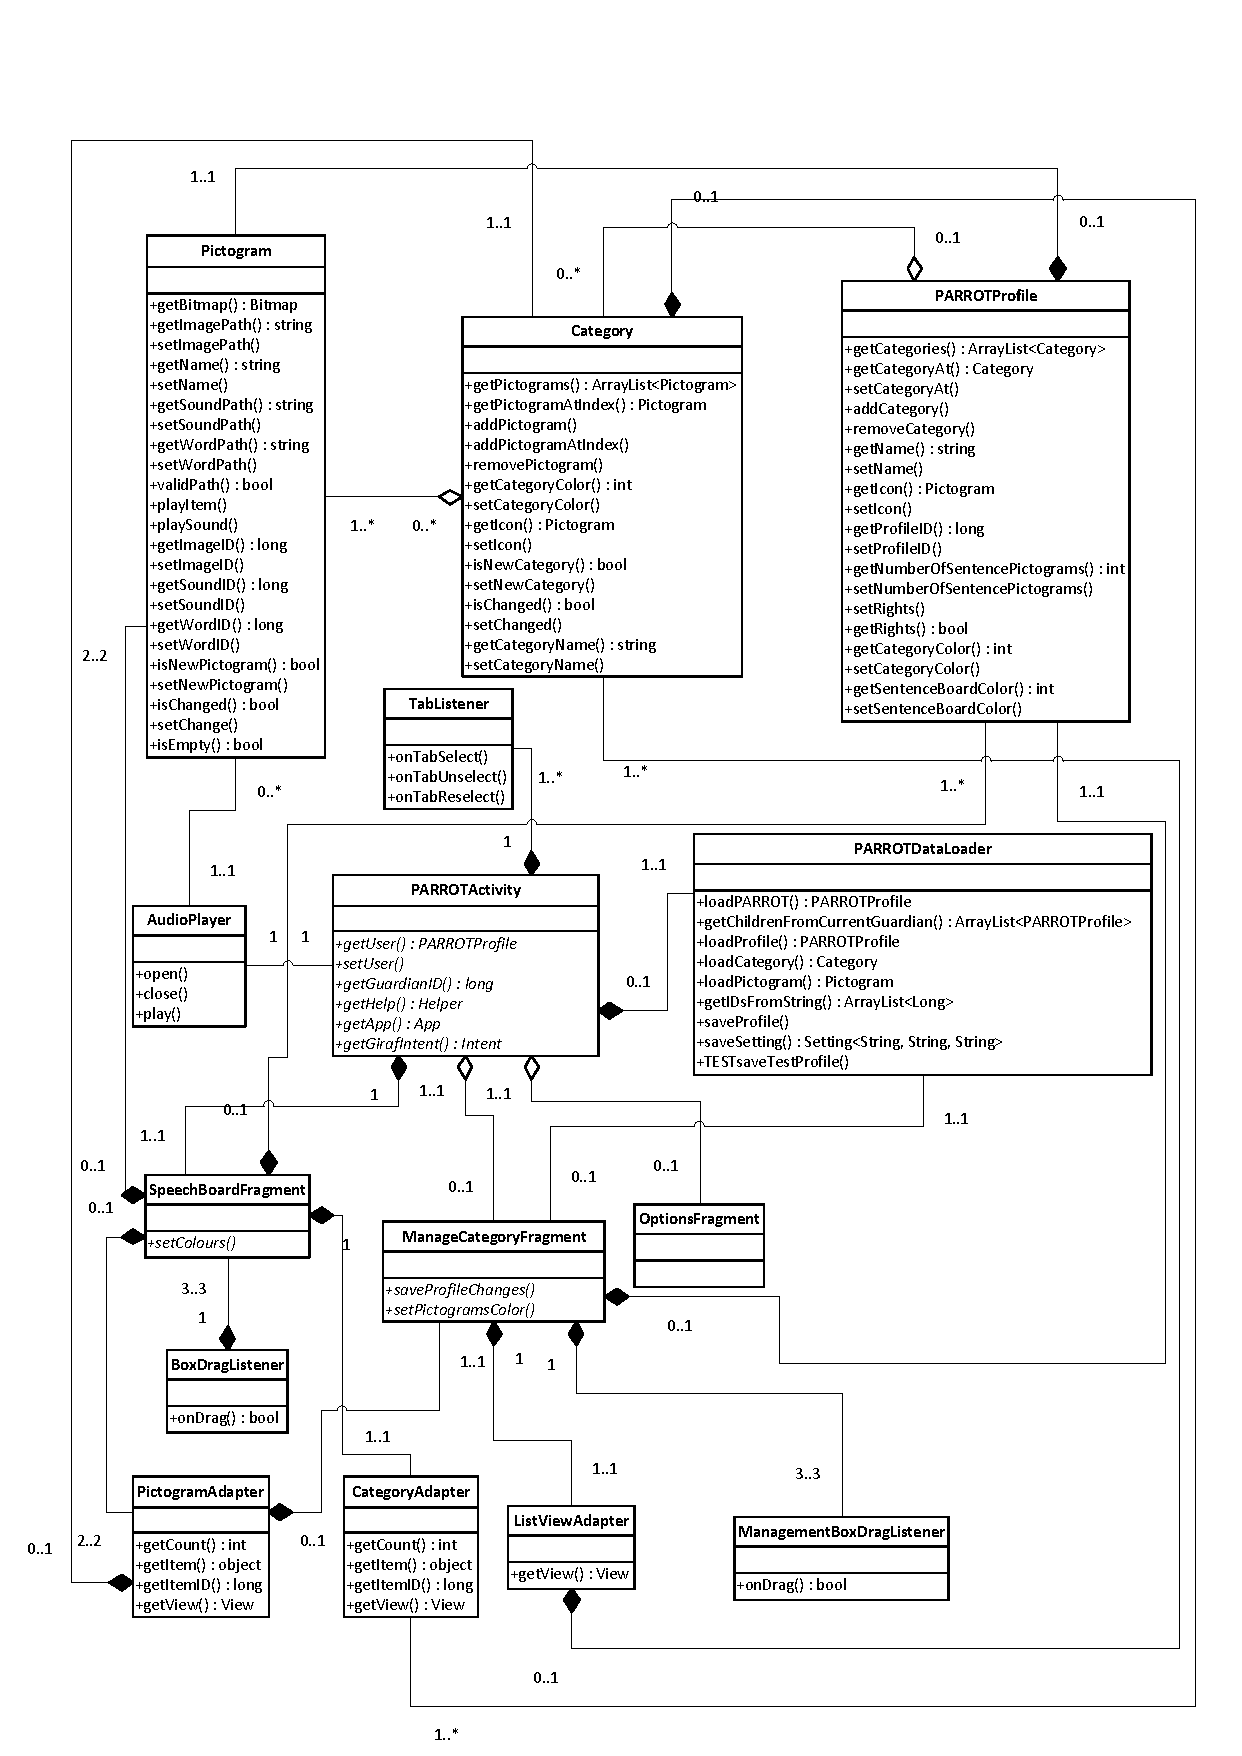
\includegraphics[width=1.0\textwidth]{input/images/ClassUMLPARROTPDF.pdf}
	\caption{UML Diagram of PARROT. Filled diamonds are composition, empty diamonds are aggregation.}
	\label{fig:ClassUMLPARROTPDF}
\end{figure}


\InputIfFileExists{input/Implementation/parrotxml}{}{}
\InputIfFileExists{input/Implementation/DragAndDrop}{}{}
\InputIfFileExists{input/Implementation/Sound}{}{}
\InputIfFileExists{input/Implementation/actionbar_tabs}{}{}
\InputIfFileExists{input/Implementation/Colour}{}{}
\InputIfFileExists{input/Implementation/Show_Pictograms}{}{}
\InputIfFileExists{input/Implementation/SentenceBoard}{}{}
\InputIfFileExists{input/Implementation/ManagingCategories}{}{}
\InputIfFileExists{input/Implementation/Database}{}{}\\
\\
\textit{The software for the PARROT application was presented in this chapter and the Source Code for the features and the design has been described. Now that the application is in a working state and running, it is possible to make the tests of the Source Code.}